\chapter{El modelo actuarial de la renta vitalicia inmediata}
\label{cap:modelo}

Este capítulo define la función $\VP$ utilizada en el motor de valoración
descrito en el \cref{ap:software}. El modelo incorpora obligaciones pensionales
y convenciones de la implementación, entre ellas la discretización temporal,
las hipótesis demográficas y financieras y los recargos. El análisis posterior
caracteriza esta función para parámetros fijados; no constituye por sí mismo
una validación integral de la nota técnica ni una descripción de todos los
modelos de valoración admitidos en Colombia. Se distinguen a continuación las
prestaciones del contrato de las hipótesis y reglas particulares del cotizador.

\section{El contrato y sus coberturas}

\begin{definition}[Renta vitalicia inmediata]
Contrato de seguro de prima única mediante el cual una aseguradora, a cambio de un
capital $\KA$ entregado al inicio, se obliga a pagar una renta periódica al
pensionado y, tras su fallecimiento, a los beneficiarios con derecho reconocido,
mientras subsista ese derecho.\footnote{Definición conforme al artículo 80 de la Ley 100 de 1993, que caracteriza la renta vitalicia inmediata como la modalidad en que el afiliado contrata directamente con la aseguradora el pago de una renta mensual hasta su fallecimiento, y el pago de pensiones de sobrevivientes en favor de sus beneficiarios por el tiempo a que ellos tengan derecho.}
\end{definition}

La implementación descompone el costo del contrato en los siguientes
componentes. El amparo básico y el auxilio funerario corresponden a prestaciones;
la reserva por cambio de grupo es un recargo del modelo cuya cuantía debe
respaldarse en la nota técnica aplicable:

\begin{enumerate}[leftmargin=*]
  \item \textbf{Amparo básico.} El pago periódico de la mesada al grupo asegurado
        $Y$ mientras al menos uno de sus integrantes conserve el derecho.
  \item \textbf{Auxilio funerario.} Un pago único al fallecimiento del causante\footnote{Artículo 86 de la Ley 100 de 1993, referido al régimen de ahorro individual: el auxilio se determina a partir del salario base de cotización o de la última mesada, según corresponda, dentro de los límites de cinco y diez salarios mínimos legales mensuales vigentes.},
        acotado inferior y superiormente en función del salario mínimo.
  \item \textbf{Reserva por cambio de grupo.} Un recargo que cubre la posibilidad
        de que la composición del grupo beneficiario se modifique respecto de la
        declarada.
\end{enumerate}

A ellas se añaden los recargos por gastos de administración y expedición.

\section{Discretización y horizonte}

El modelo trabaja sobre una malla mensual. Sea $t=1,\dots,N$ el índice de mes,
con
\[
  N \;=\; \datoNMeses \quad\text{meses}\;\approx\;\datoAniosProyeccion\ \text{años},
\]
donde el primer periodo termina en el último día del mes de la fecha de
valoración. La implementación aplica además un corte general fijo:
\begin{equation}
\label{eq:vigencia}
  \nu_t \;=\; \ind_{\{t<\,\datoVigenciaCorte\}},
\end{equation}
de modo que la proyección se anula a partir del mes $\datoVigenciaCorte$
($\approx\datoAniosVigencia$ años). Este corte temporal debe distinguirse de la
extinción de la supervivencia y del derecho de cada integrante, que depende
de su edad y condición. Los pesos de los flujos pueden anularse antes del corte
general. El horizonte finito permite acotar el conjunto de quiebres candidatos
de $\VP$; no implica que todos ellos produzcan un salto efectivo
(\cref{thm:quiebres}).

\section{Proyección de la mesada}
\label{sec:proyeccion-mesada}

\subsection{Esquema de indexación en tres tramos}

La mesada se reajusta anualmente. El modelo no usa una tasa única sino un esquema
de tres tramos, que refleja la práctica de proyección macroeconómica: el primer
año se toma la inflación observada o proyectada de corto plazo, el segundo la de
la encuesta de expectativas, y a partir del tercero la meta de largo plazo del
banco central.\footnote{La meta de inflación de largo plazo del Banco de la República de Colombia es del tres por ciento anual, con un rango de tolerancia de un punto porcentual. Las expectativas de corto y mediano plazo se toman de la encuesta mensual de expectativas de analistas económicos que publica el propio banco.}

\begin{definition}[Factor de indexación acumulado]
\label{def:factor-indexacion}
Sean $\pi_1,\pi_2,\pi_\infty$ las tasas de los tramos primero, segundo y de largo
plazo, y sea $\delta\ge0$ un \emph{deslizamiento}. Para $n$ años transcurridos
desde la valoración se define
\begin{equation}
\label{eq:factor-ipc}
  \Phi_n(\delta)\;=\;
  \begin{cases}
    1, & n=0,\\[2pt]
    1+\pi_1+\delta, & n=1,\\[2pt]
    (1+\pi_1+\delta)(1+\pi_2+\delta), & n=2,\\[2pt]
    (1+\pi_1+\delta)(1+\pi_2+\delta)(1+\pi_\infty+\delta)^{\,n-2}, & n\ge3.
  \end{cases}
\end{equation}
Se escribe $\tau_t=\Phi_{n(t)}(0)$ para el factor de la mesada y
$\phi_t=\Phi_{n(t)}(\delta)$ para el del salario mínimo, donde $n(t)$ es el número
de años calendario transcurridos hasta el mes $t$.
\end{definition}

El \emph{deslizamiento} $\delta$ es el excedente con que el salario mínimo legal
crece por encima de la inflación, y responde a la política de aumentos reales del
salario mínimo. En la proyección se toma $\delta\ge0$ como hipótesis sobre esa
trayectoria futura. Si $\delta>0$, se separan progresivamente $\phi_t$ y
$\tau_t$ y se dispersan los umbrales de distintos años. Si $\delta=0$,
los operadores de máximo y recorte conservan sus umbrales, pero estos
coinciden en uno, cinco y diez salarios mínimos.

\subsection{Piso legal del salario mínimo}

Sea $S_0$ el salario mínimo vigente y $S_t=S_0\,\phi_t$ su proyección. La
normativa garantiza que ninguna mesada sea inferior al salario mínimo, de modo que\footnote{Artículo 35 de la Ley 100 de 1993: el monto mensual de la pensión mínima de vejez o jubilación no podrá ser inferior al valor del salario mínimo legal mensual vigente. La indexación anual de las mesadas por la variación del índice de precios al consumidor está establecida en el artículo 14 de la misma ley.}
la mesada efectiva del mes $t$ generada por una mesada inicial $M$ es
\begin{equation}
\label{eq:mesada-piso}
  M_t(M) \;=\; \max\bigl\{\,M\,\tau_t,\;S_t\,\bigr\}.
\end{equation}

\begin{remark}[Una distinción de casos en la implementación]
\label{rem:rama-smlv}
El motor de producción selecciona el factor de crecimiento por una distinción de
casos: usa $\phi_t$ (con deslizamiento) si $M=S_0$ exactamente, y $\tau_t$ (sin
deslizamiento) en caso contrario. Como se demuestra en la
\cref{prop:continuidad-rama}, esta distinción \emph{no afecta el valor} de
$\VP$ --- el piso de \cref{eq:mesada-piso} la absorbe --- pero sí afecta la
fórmula de la derivada en el punto $M=S_0$. Corresponde a la recomendación~R2 de la
\cref{sec:hallazgos-codigo}.
\end{remark}

\subsection{Número de mesadas por año}

Los sistemas pensionales colombianos pagan $13$ o $14$ mesadas anuales según el
régimen\footnote{La mesada catorce fue suprimida para las pensiones causadas a partir del 31 de julio de 2011 por el Acto Legislativo 01 de 2005, con excepción de quienes se pensionaran antes de esa fecha con una mesada inferior a tres salarios mínimos. Ambos regímenes coexisten, por lo que el modelo debe soportar los dos.}. Sea $\kappa_t\in\{0,1,2\}$ el número de pagos del mes calendario
correspondiente a $t$, con $\kappa=2$ en noviembre y, en el régimen de $14$
mesadas, también en junio. El pago total del mes es $M_t(M)\,\kappa_t$.

\section{Contingencia multivida}

Sea $Y$ el grupo asegurado. Para cada $y\in Y$ se construye la supervivencia
mensualizada $\npx{t}{y}$ mediante \cref{eq:npx-producto}, aplicando:

\begin{itemize}[leftmargin=*]
  \item un \emph{factor de aplicabilidad} $\alpha_y$ ($0{,}70$ para el causante
        válido, $0{,}95$ para beneficiarios válidos, $1$ para inválidos), aplicado
        como ajuste adicional a la mortalidad de partida. Su magnitud procede
        del cotizador y requiere justificación mediante experiencia o nota
        técnica; no se deduce de la selección del colectivo por sí sola
        (\cref{sec:var-demograficas});
  \item \emph{factores de mejora de longevidad} $(1-r_x)^{a}$, donde $a$ es el
        número de años transcurridos desde el año base de la tabla, acotado a
        $30$;
  \item una \emph{duración del derecho} $\DURA_y$, que trunca la supervivencia
        efectiva: vitalicia para cónyuge y padres, hasta los $25$ años para hijos
        válidos, vitalicia para hijos inválidos, y hasta $20$ años para cónyuges
        temporales\footnote{Artículo 74 de la Ley 100 de 1993 y sus modificaciones. El cónyuge o compañero permanente menor de treinta años sin hijos con el causante recibe la pensión de sobrevivientes de forma temporal, por veinte años; los hijos conservan el derecho hasta los dieciocho años, o hasta los veinticinco si acreditan escolaridad, o de forma vitalicia si son inválidos.}.
\end{itemize}

Con ello, el factor de contingencia del amparo básico es
\begin{equation}
\label{eq:conab-modelo}
  \CONAB(t)\;=\;1-\prod_{y\in Y}\bigl(1-\npx{t}{y}\bigr),
\end{equation}
de acuerdo con la \cref{prop:conab}. La \cref{fig:supervivencia} muestra estas
curvas calculadas con las tablas reales.

\begin{figure}[H]
\centering
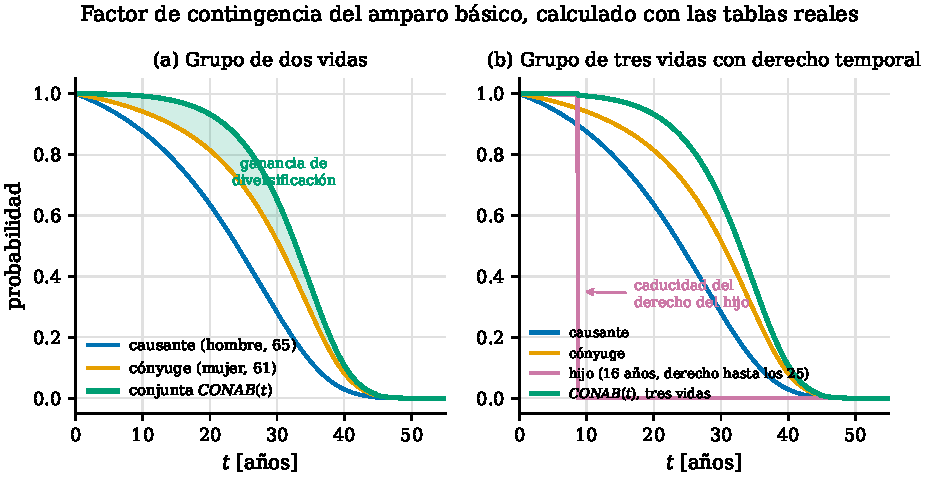
\includegraphics[width=\textwidth]{figuras/fig_supervivencia}
\caption[Factor de contingencia del amparo básico]{Supervivencia individual y
conjunta calculada con las tablas colombianas RV-08. La curva conjunta domina a
las individuales: el contrato dura, en esperanza, más que cualquiera de las vidas
por separado. En el panel (b), el derecho temporal del hijo caduca a los $25$ años
y su curva cae a cero, sin que $\CONAB$ se vea prácticamente afectado porque los
padres siguen vivos con alta probabilidad.}
\label{fig:supervivencia}
\end{figure}

\section{Descuento financiero}

Sea $i$ la tasa de interés técnico \emph{real} y $\{\pi^m_t\}$ la sucesión de
inflaciones mensuales implícitas del esquema de tres tramos. La tasa nominal
mensual del periodo $t$ es
\begin{equation}
\label{eq:tasa-nominal}
  j_t \;=\; (1+\pi^m_t)\,(1+\varepsilon_t)-1,
  \qquad
  \varepsilon_t=(1+\iota_t)^{1/12}-1,
\end{equation}
donde $\iota_t$ es la tasa \emph{forward} anual real obtenida de la curva
\emph{spot}\footnote{La relación telescópica entre tasas \emph{spot} y \emph{forward} es una identidad de no arbitraje, no una hipótesis de modelación: expresa que invertir a $t$ años debe rendir lo mismo que invertir a $t-1$ años y reinvertir un año más al tipo pactado hoy para ese periodo.} $\{i_t\}$ mediante la relación telescópica
$1+\iota_t=(1+i_t)^t/(1+i_{t-1})^{t-1}$. El factor de descuento acumulado es
\begin{equation}
\label{eq:descuento}
  v_t\;=\;\prod_{u=1}^{t-1}\frac{1}{1+j_u},\qquad v_1=1.
\end{equation}
Si la curva es plana, $i_t\equiv i$, entonces $\iota_t\equiv i$ y
\cref{eq:descuento} se reduce a la fórmula usual. La \cref{fig:descuento} muestra
la estructura temporal empleada.

\begin{figure}[H]
\centering
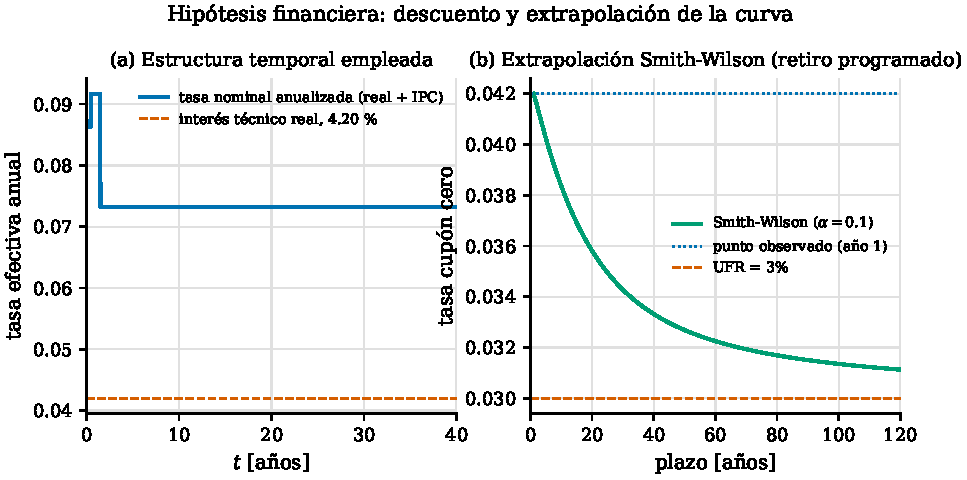
\includegraphics[width=\textwidth]{figuras/fig_descuento}
\caption[Estructura temporal de descuento]{Estructura temporal de tasas empleada
en la valoración. En el panel (a), la tasa nominal combina el interés técnico real
constante del \datoInteresRP\% con el esquema de inflación en tres tramos; la
transición entre tramos es visible en los primeros tres años. El panel (b) muestra
una ilustración de la extrapolación de Smith-Wilson, disponible en el motor
pero desactivada en la configuración de referencia
(\cref{cap:retiro}).}
\label{fig:descuento}
\end{figure}

\section{La función de valoración}

\subsection{Amparo básico}

Reuniendo \cref{eq:mesada-piso,eq:conab-modelo,eq:descuento} y aplicando el
\cref{cor:vp-renta}:
\begin{equation}
\label{eq:rab}
  \RAB(M)\;=\;\sum_{t=1}^{N}\max\{M\tau_t,\;S_t\}\;\nu_t\,\kappa_t\;\CONAB(t{+}1)\;v_{t+1}.
\end{equation}

\subsection{Auxilio funerario}

El auxilio funerario se paga al fallecimiento del causante y su cuantía es la
mesada vigente, acotada entre $5$ y $10$ salarios mínimos proyectados:
\begin{equation}
\label{eq:auf-cuantia}
  A_t(M)\;=\;
  \begin{cases}
    5S_t, & M_t(M)\le 5S_t,\\
    M_t(M), & 5S_t<M_t(M)\le 10S_t,\\
    10S_t, & M_t(M)>10S_t,
  \end{cases}
  \;=\;\med\bigl(5S_t,\;M_t(M),\;10S_t\bigr).
\end{equation}
Su valor presente actuarial es
\begin{equation}
\label{eq:auf}
  \AUF(M)\;=\;\sum_{t=1}^{N} A_t(M)\;\nu_t\;q^{(c)}_t\;\npx{t}{c}\;v_{t+1},
\end{equation}
donde $c$ denota al causante y $q^{(c)}_t$ su probabilidad de fallecimiento en el
mes $t$.

\begin{remark}
La forma $\med$ de \cref{eq:auf-cuantia} es la que produce la pérdida de
convexidad del \cref{thm:no-convexidad}. Obsérvese que el $\med$ actúa sobre
$M_t(M)$, que a su vez ya contiene un $\max$: la composición
$\med(5S_t,\max(M\tau_t,S_t),10S_t)$ es lineal a trozos con \emph{tres} quiebres
potenciales por periodo, aunque el primero de ellos, en $M\tau_t=S_t$, es inactivo
porque $S_t<5S_t$ y el $\med$ ya está saturado por abajo allí.
\end{remark}

\subsection{Recargos y reserva matemática}

Sea $\gamma$ el porcentaje de reserva por cambio de grupo y $g$ el de recargo de
gastos. Se define la \emph{base de reserva}
\begin{equation}
\label{eq:base}
  B(M)\;=\;(1+\gamma)\,\RAB(M)\;+\;\AUF(M),
\end{equation}
y la \emph{reserva matemática}, que es la función de valoración objeto de este
trabajo,
\begin{equation}
\label{eq:vp}
  \boxed{\;\VP(M)\;=\;\frac{B(M)}{1-g}\;=\;\frac{(1+\gamma)\,\RAB(M)+\AUF(M)}{1-g}.\;}
\end{equation}

La forma $B/(1-g)$ --- y no $B(1+g)$ ---\footnote{Con $g=0{,}05$, los factores son $1/(1-g)=1{,}0526316$ y $1+g=1{,}05$. La diferencia equivale aproximadamente al $0{,}263\%$ de la base $B$.} corresponde a que el recargo se define
como un porcentaje del \emph{total} y no de la base: si $R=B+gR$ entonces
$R=B/(1-g)$.

\begin{remark}[Reserva objetivo, prima y capital disponible]
En este trabajo $\VP$ designa la reserva objetivo calculada con el recargo
de gastos $g$. El motor distingue esta cantidad de la prima comercial,
que puede utilizar un recargo diferente. Por tanto, $\KA$ debe representar
el capital asignado a financiar la misma base de obligaciones y recargos
que contiene $\VP$. La igualdad $\VP(M)=\KA$ no identifica automáticamente
reserva matemática y prima comercial. La conciliación entre capital recibido,
gastos, reserva y prima requiere los términos de la nota técnica y del
contrato; no se presupone en el análisis numérico.
\end{remark}

\subsection{El problema de cotización}

\begin{definition}[Problema de cotización]
\label{def:problema}
Dado un capital $\KA>0$, hallar una mesada admisible $M^*\ge S_0$ tal que
\begin{equation}
\label{eq:problema}
  f(M^*)\;=\;\VP(M^*)-\KA\;=\;0.
\end{equation}
\end{definition}

Para estudiar la estructura de la valoración se utiliza también su extensión
a $M\ge0$, definida por las mismas fórmulas. La multiplicidad de raíces en
$[0,S_0]$ pertenece a ese dominio ampliado. En el dominio admisible, si
$\KA=\VP(S_0)$ y $\VP$ es estrictamente creciente por encima de $S_0$,
la solución es únicamente $M^*=S_0$.

\begin{remark}[Convención de signo]
El motor de producción define la función objetivo como $\KA-\VP(M)$, que es
\emph{no creciente}. En este trabajo se adopta la convención opuesta,
$f=\VP-\KA$, que es \emph{no decreciente} y estrictamente creciente por encima
de $S_0$, porque es la que permite aplicar sin cambios
de signo la teoría de métodos para funciones monótonas crecientes. La raíz es
evidentemente la misma.
\end{remark}

\section{Descomposición del valor presente}

La \cref{fig:flujos} descompone $\VP$ en sus tres factores para una póliza
concreta: la mesada proyectada, que crece con la indexación; el flujo esperado,
que es el producto de la mesada por la contingencia y por eso primero crece y
luego decae; y el flujo descontado, cuya área es exactamente $\VP$.

\begin{figure}[H]
\centering
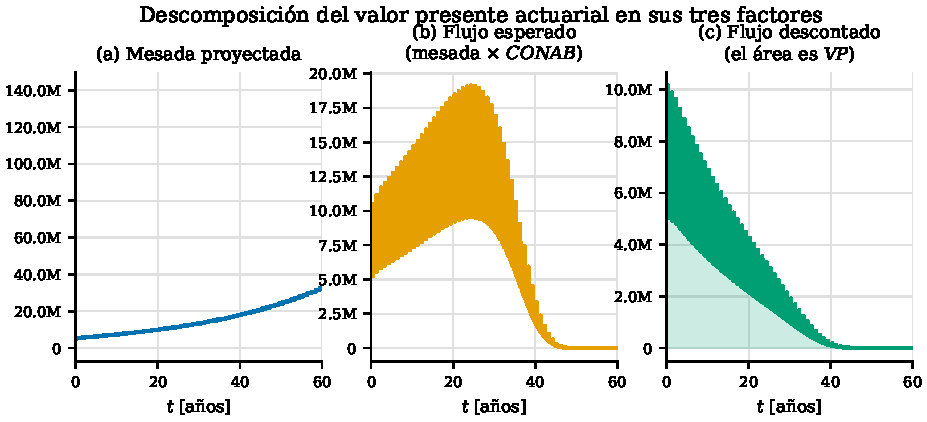
\includegraphics[width=\textwidth]{figuras/fig_flujos}
\caption[Descomposición del valor presente actuarial]{Descomposición del valor
presente actuarial. La forma del flujo descontado --- un máximo temprano seguido de
un decaimiento --- es la que determina la duración de Macaulay del contrato y, como
se verá en la \cref{sec:interpretacion-subdif}, la magnitud de la derivada
$\VP'$.}
\label{fig:flujos}
\end{figure}

\section{Forma canónica}

Todo el capítulo se resume en la siguiente observación, que es el punto de partida
del análisis estructural.

\begin{proposition}[Forma canónica de la función de valoración]
\label{prop:forma-canonica}
La función $\VP$ definida en \cref{eq:vp} admite la representación
\begin{equation}
\label{eq:canonica}
  \VP(M)\;=\;\sum_{t=1}^{N} w_t\,\max\{a_tM,\,b_t\}
            \;+\;\sum_{t=1}^{N} c_t\,\med\bigl(5b_t,\;a_tM,\;10b_t\bigr),
\end{equation}
con coeficientes
\begin{align*}
  w_t&=\frac{(1+\gamma)\,\nu_t\kappa_t\,\CONAB(t{+}1)\,v_{t+1}}{1-g}\ \ge 0,\\
  c_t&=\frac{\nu_t\,q^{(c)}_t\,\npx{t}{c}\,v_{t+1}}{1-g}\ \ge 0,
\end{align*}
\[
  a_t=\tau_t>0,\qquad b_t=S_t=S_0\phi_t>0,
\]
todos ellos \textbf{independientes de $M$}.
\end{proposition}
\begin{proof}
Sustitúyanse \cref{eq:rab,eq:auf} en \cref{eq:base,eq:vp} y agrúpense los factores
que no dependen de $M$. Para el segundo sumando obsérvese que
\[
\med(5S_t,\max(a_tM,b_t),10S_t)=\med(5b_t,a_tM,10b_t),
\]
ya que
$\max(a_tM,b_t)<5b_t$ si y solo si $a_tM<5b_t$ (porque $b_t<5b_t$), y análogamente
para la cota superior.
\end{proof}

La ecuación \cref{eq:canonica} exhibe a $\VP$ como una \emph{combinación cónica finita de
máximos y recortes de funciones afines}. Toda la estructura del problema está
contenida en esa frase, y el capítulo siguiente la desarrolla.
